\section{Architecture du site web}
\label{sec:architecture}

\paragraph{}Dans cette section, nous pr�sentons l'architecture du site web r�alis�.
\subsection{Architecture physique}
\label{sec:archiphys}

\paragraph{} L'architecture physique du site web est divis� en 4 parties:
\begin{itemize}
\item Les pages web: � la racine du site web
\item Les fonctions php: dans les librairies dans le dossier "lib" ainsi que dans le dossier "include"
\item Les differentes ressources: dans les dossier "res" et "img"
\item Le style du site: dans les dossier "css" et "police"
\end{itemize}

\begin{figure}[H]
	\centering
		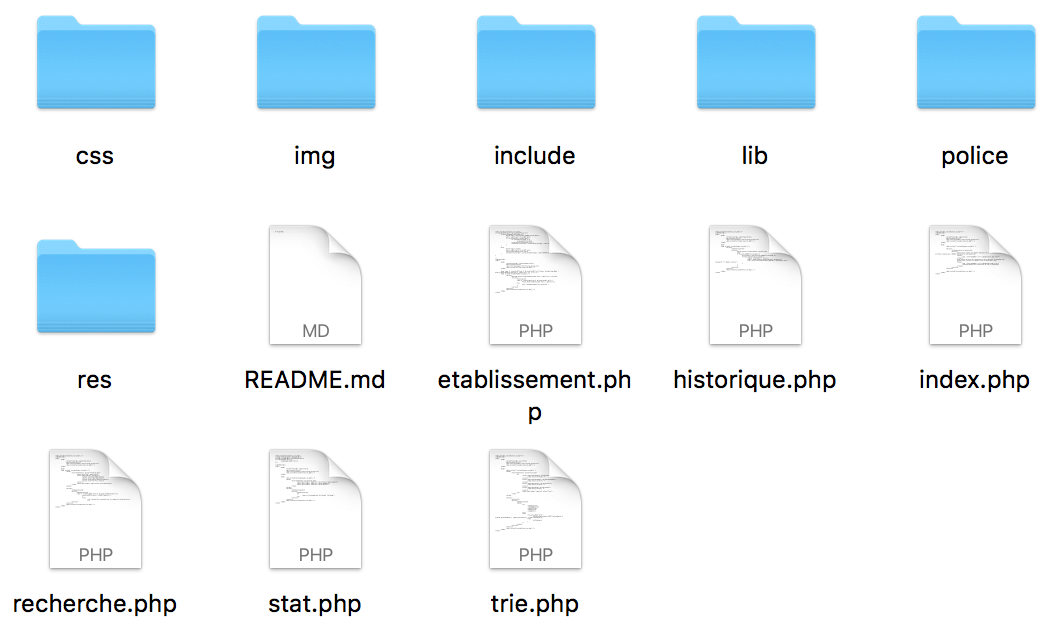
\includegraphics[width=900]{img/archi_phys.png}
		\caption{Architecture Physique du site web}
	\label{fig:archiphys}
\end{figure}

\subsection{Architecture Logique}
\label{sec:archilog}

\paragraph{}Le site web est construit de telle mani�re � ce que chaque page soit accessible � partir de n'importe quelle autre page. Aisni chaque page est directement accessible via la barre de navigation pr�sente en haut de chaque page, seul la page "�tablissement" est accessible via un lien pouvant �tre obtenu par une recherche d'�tablissement ou sur la page de tri.

\begin{figure}[H]
	\centering
		
\includegraphics[width=900]{img/header.png}
		\caption{Barre de navigation}
	\label{fig:navbar}
\end{figure}